\documentclass[a4paper, 11pt]{article}

% draftwatermark
\usepackage{draftwatermark}
\SetWatermarkText{\tt DRAFT}
\SetWatermarkLightness{.8}
\SetWatermarkScale{10}

% urls
\usepackage{url}

% figures
\usepackage{array}
\usepackage{float}
\usepackage{wrapfig}

% tables
\usepackage{booktabs}
\usepackage{tabu}

% margins
\usepackage{graphicx}

% source code
\usepackage{xcolor}
\usepackage{listings}
\lstdefinestyle{customc}{
  belowcaptionskip=1\baselineskip,
  breaklines=true,
  frame=L,
  xleftmargin=\parindent,
  language=C,
  showstringspaces=false,
  basicstyle=\footnotesize\ttfamily,
  keywordstyle=\bfseries\color{green!40!black},
  commentstyle=\color{purple!40!black},
  identifierstyle=\color{blue},
  stringstyle=\color{orange},
}

\lstdefinestyle{customasm}{
  belowcaptionskip=1\baselineskip,
  frame=L,
  numbers=left,
  numberstyle=\ttfamily,
  xleftmargin=\parindent,
  language=[x86masm]Assembler,
  basicstyle=\footnotesize\ttfamily,
  commentstyle=\color{gray},
}

% language (set correct hypenation)
\usepackage[italian]{babel}
\usepackage{textgreek}

% to fix macros
\usepackage{xspace}
% commands
% macro for project name
\newcommand{\prj}{Z80\textmu PC\xspace}

% invert signal (not, active low)
\newcommand{\inv}[1]{\(\overline{\mbox{#1}}\)}
 
% metadata
\title{\prj Single Board \\ Computer Development }
\author{Naoki Pross}

% document 
\begin{document}

\maketitle
\begin{abstract}

    Lo Zilog Z80 \`e un processore a 8 bit che fu introdotto nel 1976 ed ebbe
    un grandissimo successo nel mondo dell'elettronica e dell'informatica
    dagli anni 70 a 90. In memoria di questo pioniere dell'industria dei
    sistemi informatici questo progetto documenta la realizzazione di un
    microcomputer a scopo generico a base di esso. L'obiettivo primario
    dunque \`e di realizzare una scheda simile ad una motherboard dei
    computers venduti all'epoca completa di RAM, ROMs, interfacce seriali e
    altri circuiti di supporto. Successivamente per l'aspetto software il
    progetto deve implementare i drivers per ogni circuito presente sulla
    scheda in modo da semplificare la programmazione. L'obiettivo opzionale
    del progetto, una volta terminata la costruzione hardware, \`e di
    realizzare una kernel monolitica che offre funzioni minimali simili ad un
    sistema UNIX, quali processi, filesystem, memory management e drivers.

\end{abstract}

\break
\tableofcontents
\break

%-----------------------------------------------------------------------------
\section{Hardware}

\subsection{Specifiche tecniche dello Z80}
Lo Z80 \`e un processore molto minimalistico se paragonato a ci\`o che si
trova oggi sul mercato dei microcontrollori. Per il progetto \prj la CPU in
uso \`e il modello originale Zilog Z8400 che non dispone di moduli aggiuntivi
integrati come i modelli SoC odierni. La scelta di una CPU tanto semplice \`e
la conseguenza del design didattico del progetto, inoltre senza alcun
dispositivo interno lo Z8400 si presenta con un address space completamente
vuoto, ad eccezzione del punto d'inizio e i vettori di reset.

Lo Z80 utilizza I/O paralleli sia per la lina a 16 degli indizzi che per la
linea dati a 8 bit e dispone di 6 registri 8 bit ad utilizzo generico
combinabili in coppie per ottenere un valore a 16 bit. Per il controllo dei
dispositivi esterni, come lettura e scrittura esso possiede delle linee di
controllo dedicate come {\tt\inv{RD}}, {\tt\inv{WR}}, {\tt\inv{MREQ}}, ecc. In
quanto instruction set, lo Z80 ha 158 istruzioni possibili di cui 78 sono un
sottoinsieme dello 8080A, architettate per poter mantere una
retrocompatiblit\`a.

\begin{table}[ht]\centering
\caption{Riassunto delle specifiche}

\begin{tabular}{ l l }
    \toprule
    Dimensione Indirizzi    & 16 bit \\
    Dimensione Dati (word)  & 8 bit \\
    Spazio Indirizzabile    & 64 KB \\
    Registri Generici 8 bit & 6 ({\tt A..F}) \\
    Registri 16 bit         & 2 ({\tt SP, PC}) \\
    Clock speed             & 8 MHz, 6MHz, 4MHz, 2.5MHz \\
    \bottomrule
\end{tabular}
\end{table}

\subsection{Componenti e modello di design}
Il minimo necessario per far funzionare uno Z80 sono una {\tt RAM} ed una
{\tt ROM}, ma avendo a disposizione altri dispositivi I/O lo \prj dispone
anche di una porta seriale, di una porta parallela e di un counter timer;
Hardware che si presenta normalmente all'interno di microcontrollori odierni.

\begin{table}[h!]\centering
\caption{Lista dei componenti}
\begin{tabular}{ >{\tt}p{.1\textwidth} >{\tt\bfseries}p{.2\textwidth} >{\footnotesize}p{.6\textwidth} }
    \toprule
    ROM & M28C64    & EEPROM da 8KB x 8 bit (64K) per il BIOS / Bootloader /
                      OS installata doppia per avere 16KB \\
    RAM & HM62256B  & SRAM da 32KB x 8bit (256K) \\
    CTC & Z8430     & Counter timer circuit ufficiale di Zilog a 4 canali
                      programmabili \\
    PIO & Z8420     & Parallel input/output controller di Zilog per avere un
                      intefaccia digitale con due porte da 8 bit \\
    MMU & M4-32/32-15JC & CPLD programmabile che implementa una memory 
                          management unit semplificata in grado di gestire i 
                          5 bit pi\`u significativi della linea di indirizzi \\
    USART & TL16C550C & Interfaccia USART per poter comunicare utilizzando il
                        protocollo RS232 \\
    \bottomrule
\end{tabular}
\end{table}

Il design dello \prj \`e costruito sulla falsa riga di un Arduino o di un
EasyPIC con l'aggiunta di funzionalit\`a a scopo didattico quali; la
possiblit\`a di cambiare la velocit\`a di clock tra 4MHz, 200Hz o manuale
(mediante un bottone sulla scheda) e una serie di display a 7 segmenti per
vedere in tempo reale i valori sui bus degli indirizzi e dei dati.
\begin{center}
\begin{tabular}{ >{\bfseries}r p{.8\textwidth} }
    0Hz     & Il clock manuale \`e un bottone che permette di creare
              le pulsazioni, per poter analizzare ogni istruzione \\
    200Hz   & Mediante un classico circuito con un LM555 si ha un clock
              per eseguire i programmi a velocit\`a rallentata \\
    4MHz    & Clock per esecuzione a velocit\`a piena (normale)
\end{tabular}
\end{center}

\subsection{Schema a blocchi}
\begin{figure}[H]
    \centering
    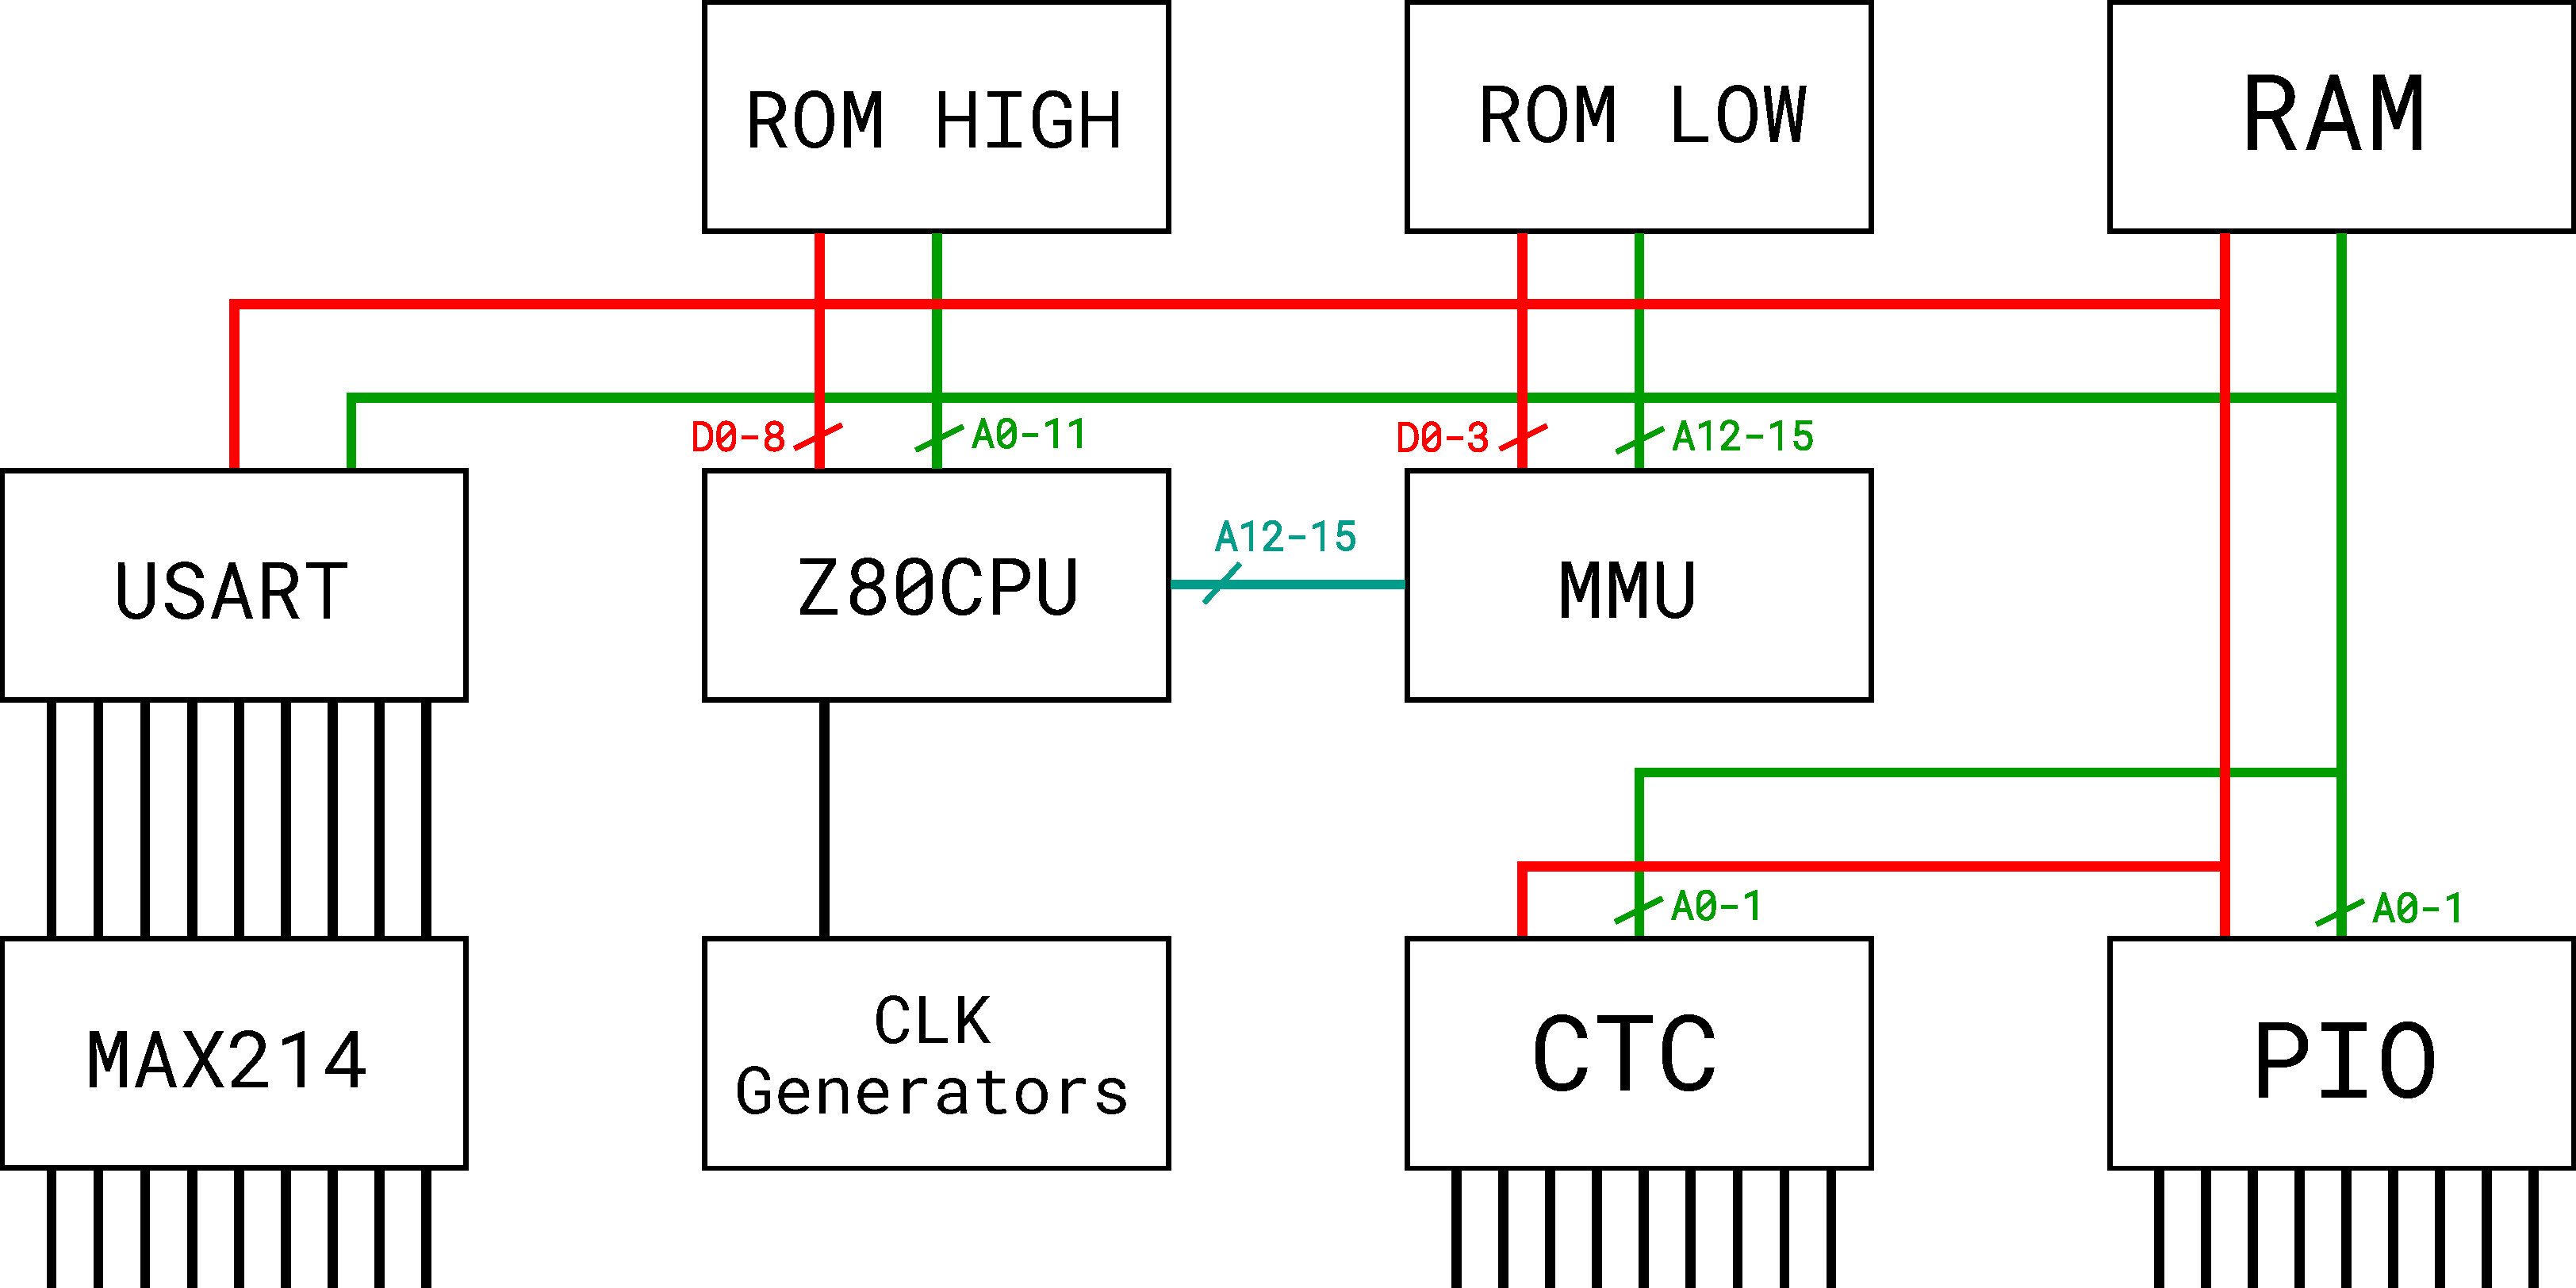
\includegraphics[width=\textwidth]{res/block_diagram}
    \caption{Schema a blocchi del \prj}
\end{figure}

% TODO
\subsubsection{Implementazione dei generatori di clocks}

\subsubsection{Uscite verso l'esterno (DIN 41612)}
Per poter estendere lo \prj a lato \`e presente un connettore {\tt DIN 41612}
per poter interfacciare schede di estensione della funzionali\`a siccome il
progetto lascia liberi la maggior parte dei 16KB dell'\emph{i/o space}, ovvero
la parte di address space in cui \`e previsto di mappare dispositivi esterni.
\begin{table}[H]
\caption{Mappatura dei segnali nel connettore DIN 41612}
\vspace{5pt}
\resizebox{\textwidth}{!}{\begin{tabu}{l l l l l l l l l l l l l l l l}
    \toprule
    1 & 2 & 3 & 4 & 5 & 6 & 7 & 8 & 9 & 10 & 11 & 12 & 13 & 14 & 15 & 16 \\
    \midrule
    \rowfont{\tt}
    GND & GND & VCC & VCC & D0 & D1 & D2 & D3 & D4 & D5 & D6 & D7 & A0 & GND & A2 & A1 \\
    \\
    \toprule
    17 & 18 & 19 & 20 & 21 & 22 & 23 & 24 & 25 & 26 & 27 & 28 & 29 & 30 & 31 & 32 \\
    \midrule
    \rowfont{\tt}
    A4 & A3 & A6 & A5 & A8 & A7 & A10 & A9 & 12 & A11 & A14 & A13 & & A15 & & \\
    \\
    \toprule
    33 & 34 & 35 & 36 & 37 & 38 & 39 & 40 & 41 & 42 & 43 & 44 & 45 & 46 & 47 & 48 \\
    \midrule
    \rowfont{\tt}
    \inv{RD} & & & \inv{WR} & & GND & & \inv{M1} & & GND & \inv{INT} & \inv{RST} & \inv{MREQ} & \inv{NMI} & \inv{HALT} & \inv{IORQ}\\
    \\
    \toprule
    49 & 50 & 51 & 52 & 53 & 54 & 55 & 56 & 57 & 58 & 59 & 60 & 61 & 62 & 63 & 64 \\
    \midrule
    \rowfont{\tt}
    \inv{RFSH} & \inv{WAIT} & GND & & \inv{BUSREQ} & & \inv{BUSACK} & & CLK & & & & VCC & VCC & GND & GND\\
\end{tabu}}
\end{table}

% TODO
\subsection{Address space}
L'address space dello z80 \`e in grado di indirizzare 64 KB; la met\`a di
questi \`e assegnata alla RAM e un quarto \`e della ROM. La ROM \`e minore
della RAM perch\'e \`e intesa per essere un bootloader piuttosto che un vero e
proprio OS.
% TODO: redraw with xfig
\begin{figure}[H]
\centering
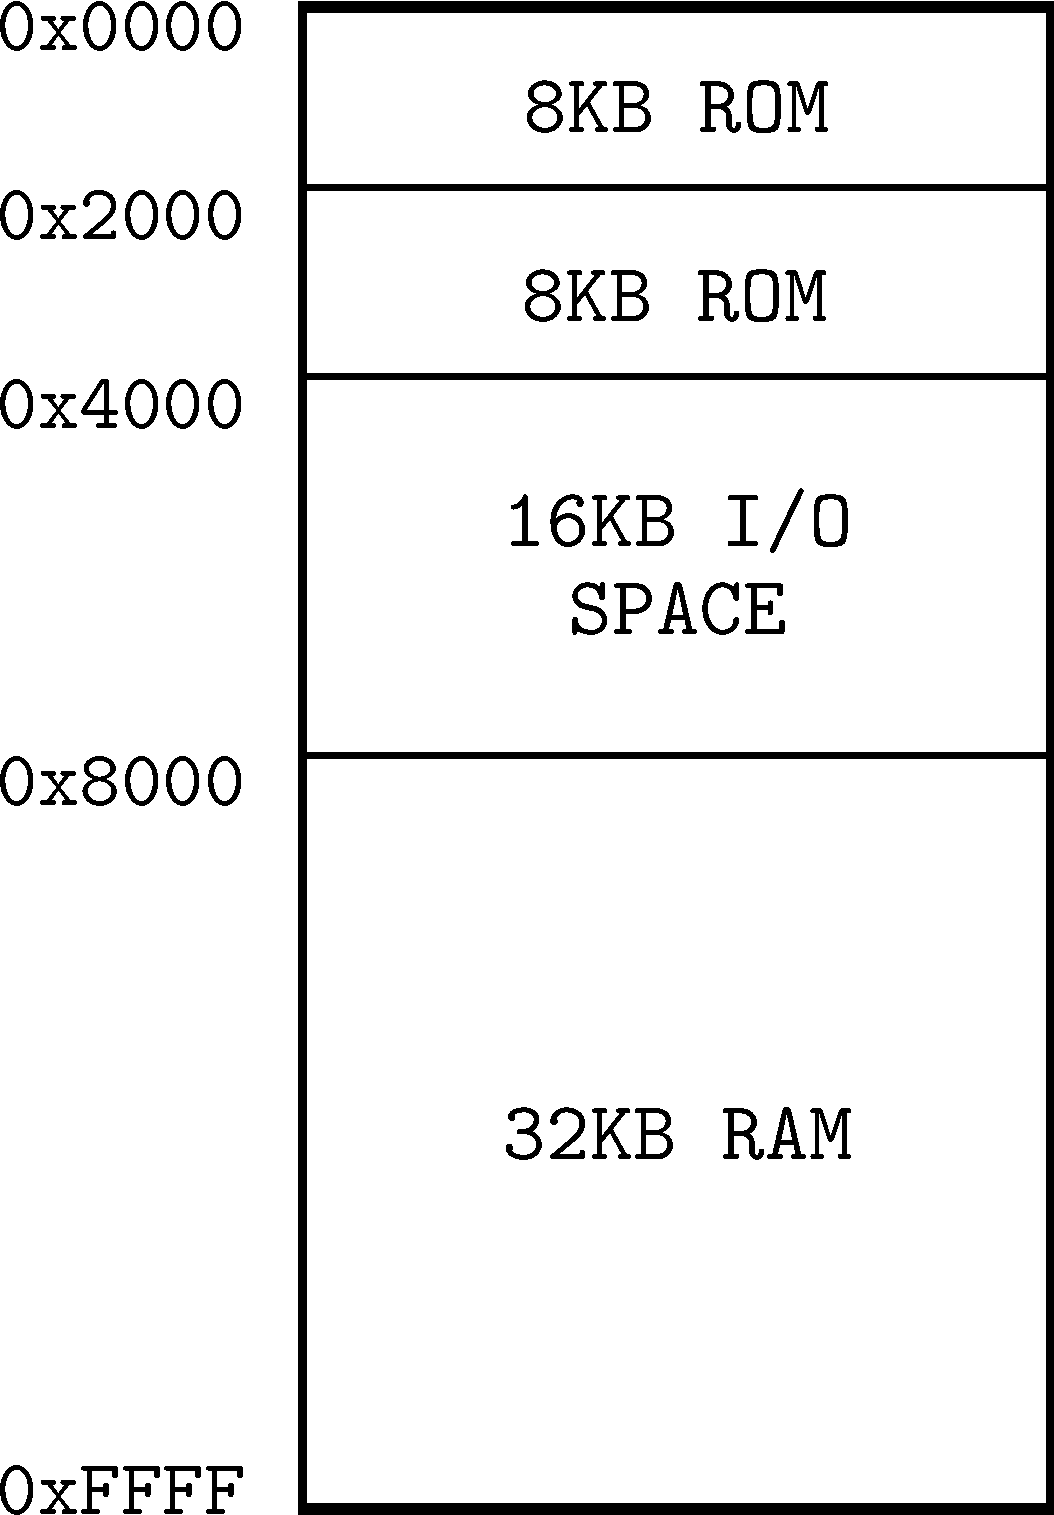
\includegraphics[height=8cm]{res/addrspace}
\end{figure}

\subsection{Memory management unit}
Alcuni modelli sucessori dello Z8400 implementavano ina MMU (Memory Management
Unit) SoC che permetteva di ampliare la dimensione dell'address space,
permettendo quindi di mappare pi\`u memorie o dispositivi separati negli stessi
indirizzi. Lo \prj per\`o cerca di imitare un architettura pi\`u simile ad un
computer X86 in cui la MMU viene utilizzata per la gestione delle \emph{pagine}
di memoria. Il concetto di pagine (pages in inglese) \`e necessario per sistemi
con un supporto per il multitasking. La conseguenza di questo design implica
per\`o che sia introdotto anche il concetto di \emph{virtual address space}
siccome, potendo reindirizzare a piacimento gli indirizzi, diventa possibile e
conveniente offrire ai programmi eseguiti la stessa struttura di memoria
indipendentemente dalla loro vera locazione in memoria.

La struttura designata per il progetto \`e la seguente. \`E resa possibile
solamente l'esecuzione di 2 programmi semi-paralleli, perch\`e
l'implementazione di uno scheduler \`e troppo complessa con il CTC a
disposizione. Si pu\`o quindi avviare due programmi ma solamente uno \`e in
esecuzione ed utilizza il 100\% del tempo della CPU. Purtroppo le limitazioni
di questo design non permettono di offrire funzionalit\`a importanti della
kernel, ma in un futuro  si potrebbe risolvere il problema estendendo la
piattaforma. Infatti grandi spazi dell'iospace sono stati lasciati liberi per
l'aggiunta di dispositivi esterni.

\begin{figure}[h!]
    \centering
    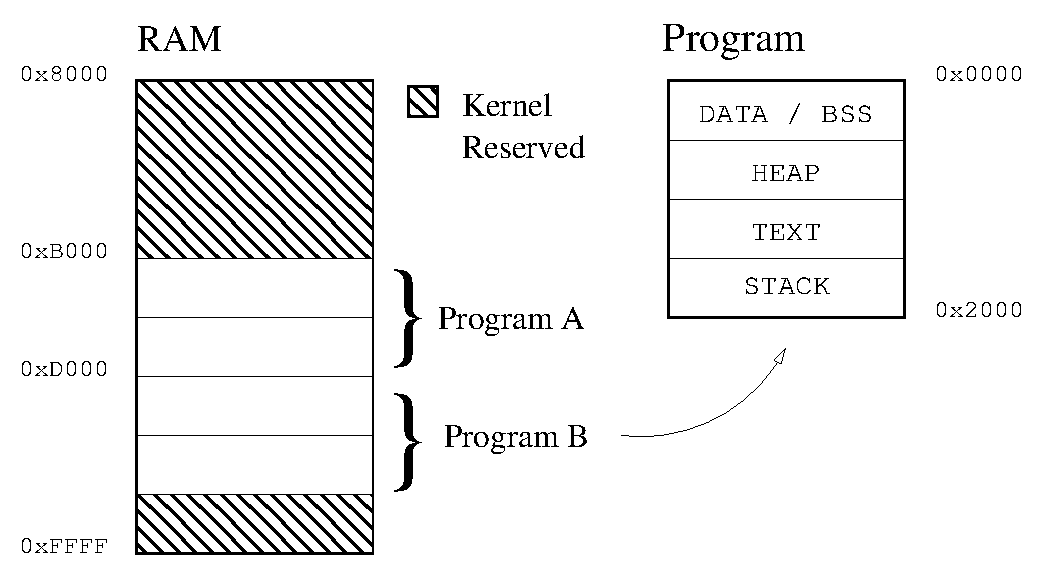
\includegraphics[height=5cm]{res/mmu_ram_map}
\end{figure}

I due programmi in `esecuzione' sono salvati nella RAM alle locazioni {\tt
0xB000} e {\tt 0xD0000} con 8 KB di RAM per uno. Per passare da un programma
all'altro la kernel offre delle system calls che modificano la \emph{page
table} all'interno della MMU in maniera da mappare l'indirizzo {\tt B000} o
{\tt D000} a {\tt 0000}.

\begin{figure}[h!]
\centering
\begin{minipage}[c]{.45\textwidth} \centering
    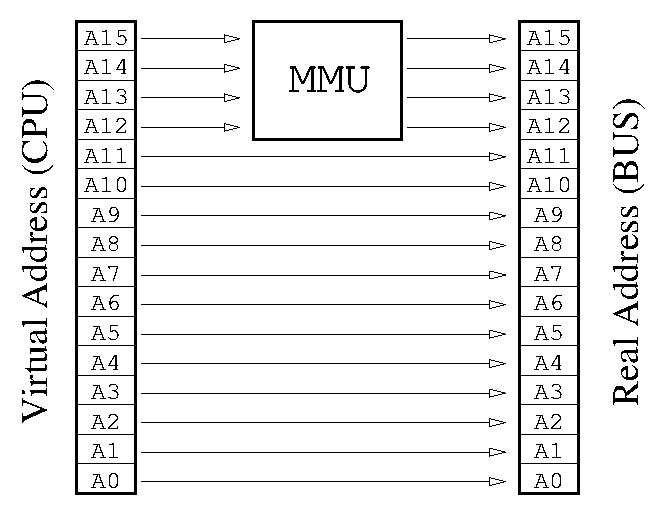
\includegraphics[width=\linewidth]{res/mmu_addr}
\end{minipage}%
\begin{minipage}[c]{.45\textwidth} \centering
\begin{verbatim}
    Example program running 
    at address 0xB000

    Virtual address
    LD (#0x1200), #0xFE

    Real Instruction
    LD (#0xC200), #0xFE
\end{verbatim}
\end{minipage}
\end{figure}

Naturalmente ci\`o significa che il programma non ha l'accesso all'iospace,
perci\`o per le operazioni con i dispositivi \`e necessario implementare un
driver nella kernel. Nel caso in cui si volesse creare dei drivers userspace la
kernel dovr\`a mettere a disposizione delle system calls che permettano di
modificare la page table in maniera indiretta.

\break
%-----------------------------------------------------------------------------
\section{Software}
\subsection{Organizzazione del codice sorgente C}
Il codice sorgente dell'intero progetto \`e contenuto nella cartella {\tt
sw/z80}.
\begin{itemize}
    \item {\tt arch} -- Contiene headers e codice essenziale che descrive la
            configurazione del dispositivo (es: gli indirizzi dei dispositivi).
    \item {\tt drivers} -- Contiene il codice per i drivers dei vari 
            dispositivi, il tutto viene compilato in una libreria statica.
    \item {\tt kernel} -- Contiene il codice della kernel monolitica del progetto.
    \item {\tt libc} -- Contiene delle implementazioni parziali di alcune 
            funzioni della standard library. Non pi\`u utilizzata.
    \item {\tt tests} -- Contiene delle test units per controllare 
            individualmente parti del progetto.
\end{itemize}

\subsection{C Toolchain}
Per compilare il codice per lo \prj \`e necessario utilizzare un \emph{cross
compiler} che sia in grado di compilare per l'architettura dello z80. Per
questo progetto si \`e scelto di utilizzare SDCC (Small Device C Compiler),
siccome \`e un progetto ancora in sviluppo attivo ed \`e utilizzato anche per
compilare in molte altre piattaforme. Per compilare un codice sorgente in un
object con SDCC per lo Z80 si utilizza il seguente comando:
\begin{verbatim}
$ sdcc -mz80 -pedantic --no-std-crt0 <crt0> \
       --allow-unsafe-read \
       -I. -c <source_file> -o <object_file>
\end{verbatim}
In cui {\tt <source\_file>} \`e il documento con il codice sorgente e {\tt
<object\_file>} \`e il nome dell'object (solitamente lo stesso del sorgente con
l'estensione {\tt .o}).  La flag {\tt --allow-unsafe-read} \`e permessa
solamente nella compilazione per Z80 e serve ad indicare al compiler che le
letture da locazioni arbitrarie di memoria sono ammesse (normalmente non lo
sono). Per linkare gli objects e generare un eseguibile si utilizza
\begin{verbatim}
$ sdcc -mz80 --no-std-crt0 <crt0> \
       --code-loc=<addr> <objects> -o <hexfile>

$ makebin -s <rom_size> -yo 1 -ya 1 <hexfile> <binary>
\end{verbatim}
Le flags {\tt -yo 1 -ya 1} specificano rispettivamente il numero di banchi di
ROM e di RAM.

\subsection{CRT0 per lo Z80}
In C il CRT0 \`e un insieme di routines che vengono eseguite prima del codice C
che servono ad inizializzare il sistema. Nel caso dello \prj \`e utilizzato per
inizializzare lo stack pointer e per indicare al linker come organizzare i
settori dell'eseguibile. Un esempio di crt0 utilizzato per il progetto:

\lstset{escapechar=@,style=customasm}
\begin{lstlisting}
    .module crt0
    .area   _HEADER (ABS)

;; Reset vectors
    .org    0
    jp  init

    ; the instruction 0xff (not written)
    ; resets to this location
    .org    0x38 
    jp init

;; main code
    .org    0x100
    .globl  _main

init:
    ;; Set stack pointer directly above top of memory.
    ld  sp,#0xffff

    ;; Start of the program
    call    _main
    jp      _exit

_exit:
    halt
    jp  _exit

;; Ordering of segments for the linker.
    .area   _HOME
    .area   _CODE
    .area   _INITIALIZER
    .area   _GSINIT
    .area   _GSFINAL

    .area   _DATA
    .area   _INITIALIZED
    .area   _BSEG
    .area   _BSS
    .area   _HEAP
\end{lstlisting}

Il CRT0 essendo scritto in assembly deve essere compilato prima utilizzando un
assembler per lo Z80, per esempio quello fornito in SDCC.\@
\begin{verbatim}
$ sdasz80 -o <crt0.s>
\end{verbatim}

Quindi l'argomento {\tt --no-std-crt0 <crt0>} per il compiler descritto
precedente non \`e assolutamente necessario ma \`e consigliato siccome permette
di avere un controllo maggiore del contenuto dell'eseguibile.

\subsection{Codice sorgente VHDL}
Il codice sorgente in VHDL per la CPLD utilizzata come address decoder e MMU, 
\`e contenuto nella cartella {\tt sw/cpld}. La toolchain utilizzata \`e quella
offerta da Lattice.

% TODO
\subsubsection{Programmazione della MMU}


\break
%-----------------------------------------------------------------------------
\section*{Glossario Tecnico}
{\def\arraystretch{1.4}
\begin{tabular}{ >{\bfseries}p{.35\linewidth} p{.65\linewidth} }

    Address Space & In informatica l'\emph{address space} \`e un intervallo di
    indirizzi che possono corrispondere a indirizzi in rete, regioni di un
    dispositivo, di una memoria o di un qualsiasi altro dispositivo fisico o
    logico.  Per questo progetto \emph{address space} si riferisce
    all'intervallo indirizzabile dal processore, ovvero \(2^{16}\) locazioni
    siccome il sistema dispone di un bus a 16 bit. \\

    Virtual Address Space & Il virtual address space \`e un livello di
    astrazione che estende l'address space utilizzato nelle architetture
    moderne (X86 / 64). In un sistema senza VAS, i programmi caricati in
    memoria `vedono' l'indirizzo in cui si trovano e devono perci\`o essere
    caricati in una regione di memoria continua. In un sistema con VAS invece
    al programma figura sempre di avere l'intero address space disponibile per
    se, e la MMU si occupa di traslare gli indirizzi virtuali in indirizzi
    reali prima che essi raggiungano l'hardware. \\

    Registro & Un registro \`e un dispositivo di memoria in cui \`e possibile
    pu\`o leggere e/o scrivere un certo valore. Normalmente in un computer /
    microcontrollore la dimensione della memoria \`e data dall'architettura,
    dunque 8, 16, 32 o 64 bits.  In questo documento viene viene comunemente
    utilizzato per riferirsi ad una memoria di un dispositivo fisico come la
    CPU o un IC seriale. \\

    Toolchain & Da Wikipedia \cite{wiki:toolchain}: In ambito software, una
    toolchain è l'insieme dei programmi (tools) usati nello sviluppo di un
    prodotto (tipicamente un altro programma o sistema di programmi). I tool
    possono essere utilizzati in catena, in modo tale che l'output di ciascun
    tool rappresenti l'input per il successivo, ma il termine è utilizzato in
    maniera più estesa per riferirsi, più in generale, a qualunque insieme di
    tool di sviluppo collegati tra loro. \\

    Stack Pointer,\newline Program Counter & Lo Stack Pointer \`e un registro a
    16 bit in cui \`e salvato l'indirizzo della fine (pi\`u in alto, ultimo
    inserito) dello stack. Il program counter, un altro registro a 16 bit
    contiene l'indirizzo da cui leggere della prossima istruzione da
    eseguire.\\

\end{tabular}}

\begin{thebibliography}{2}
\bibitem{wiki:toolchain}
    \url{https://it.wikipedia.org/wiki/Toolchain}

\bibitem{z80book}
    \textbf{Paolo Di Leo},
    Z80 Microcomputer didattico, 
    Gennaio 2016,
    Libri SANDIT,
    {\tt ISBN 978-88-6928-142-6}

\end{thebibliography}

\end{document}
